\documentclass[10pt, a4paper]{article}

\usepackage[T1]{fontenc}
\usepackage{fullpage}
\usepackage[utf8]{inputenc}
\usepackage{siunitx}
\usepackage{tikz}
\usepackage[european]{circuitikz}

\begin{document}
    \begin{center}
        \textsc{Lattice Watering}

        \vspace{\baselineskip}

        Handout

        \vspace{\baselineskip}

        Christian Müller, Jonas Heinemann, Kaan Dönmez, Valentin Pickel

        \vspace{\baselineskip}

        Software Project on Internet Communication
        
        Summer Term 2022

        Freie Universität Berlin

        \vspace{\baselineskip}

        \today{ }(latest version)
    \end{center}

    \begin{figure}[htbp!]
        \centering
        \begin{circuitikz}
            \draw (0, 0) node[left] {\(\qty{92}{\milli\ampere}, \qty{3.8}{\volt}\)}
                to[R=$\qty{200}{\ohm}$, -*] (2, 0);
            \draw (2, 0)
            to[R=\(\qty{5}{\kilo\ohm}\)] (2, -2) node[ground] {};
            \draw (4, 0) node[nigfete, tr circle] (mos) {}
            (mos.source) node[anchor=north] {}
            (mos.gate) node[anchor=east] {}
            (mos.drain) node[anchor=south] {};
            \draw (mos.inner up) -- (mos.body E out);
            \draw (mos.body E out) -- (mos.body C out);
            \draw (mos.body C out) -- (mos.body C in);
            \draw (2, 0) -- (mos.gate);
            \draw (mos.source) -- (4, -2) node[ground] {};
            \draw (mos.drain) -- (4, 2) node[circle] {P};
            \end{circuitikz}
        \caption{Circuit for the pump P.}
    \end{figure}

    Thus, we obtain:
    \[
        I_2 = \frac{\qty{5}{\volt}}{\qty{200}{\ohm}} = \qty{25}{\milli\ampere}
    \]
    And:
    \[
        I_3 = \frac{\qty{5}{\volt}}{\qty{200}{\ohm}} = \qty{25}{\milli\ampere}
    \]

    \begin{figure}[!hbtp]
        \centering
        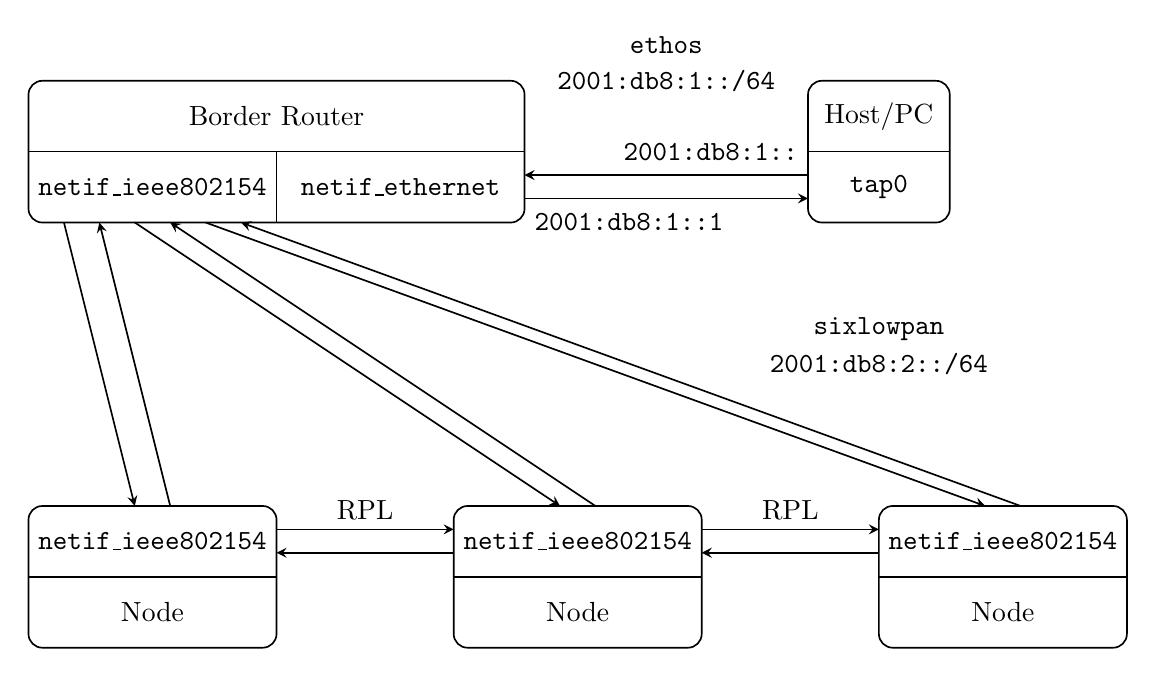
\begin{tikzpicture}[>=stealth, semithick, scale=0.9]
            \draw[rounded corners=5pt] (-1, -1) rectangle (1, 1);
            \draw[draw=none] (-1, 0) -- (1, 1) node[pos=0.5] {Host/PC};
            \draw (-1, 0) -- (1, 0);
            \draw[draw=none] (-1, 0) -- (1, -1) node[pos=0.5] {\texttt{tap0}};

            \draw[rounded corners=5pt] (-12, -1) rectangle (-5, 1);
            \draw[draw=none] (-12, 0) -- (-5, 1) node[pos=0.5] {Border Router};
            \draw (-12, 0) -- (-5, 0);
            \draw (-8.5, 0) -- (-8.5, -1);
            \draw[draw=none] (-12, 0) -- (-8.5, -1) node[pos=0.5] {\texttt{netif\_ieee802154}};
            \draw[draw=none] (-8.5, 0) -- (-5, -1) node[pos=0.5] {\texttt{netif\_ethernet}};
            \draw[->] (-1, -0.33) -- (-5, -0.33);
            \node[left] at (-1, 0) {\texttt{2001:db8:1::}};
            \node[right] at (-5, -1) {\texttt{2001:db8:1::1}};
            \node at (-3, 1.5) {\texttt{ethos}};
            \node at (-3, 1) {\texttt{2001:db8:1::/64}};
            \draw[->] (-5, -0.66) -- (-1, -0.66);

            \draw[rounded corners=5pt] (-12, -5) rectangle (-8.5, -7);
            \draw (-12, -6) -- (-8.5, -6);
            \draw[draw=none] (-12, -5) -- (-8.5, -6) node[pos=0.5] {\texttt{netif\_ieee802154}};
            \draw[draw=none] (-12, -6) -- (-8.5, -7) node[pos=0.5] {Node};

            \draw[rounded corners=5pt] (-6, -5) rectangle (-2.5, -7);
            \draw (-6, -6) -- (-2.5, -6);
            \draw[draw=none] (-6, -5) -- (-2.5, -6) node[pos=0.5] {\texttt{netif\_ieee802154}};
            \draw[draw=none] (-6, -6) -- (-2.5, -7) node[pos=0.5] {Node};

            \draw[rounded corners=5pt] (0, -5) rectangle (3.5, -7);
            \draw (0, -6) -- (3.5, -6);
            \draw[draw=none] (0, -5) -- (3.5, -6) node[pos=0.5] {\texttt{netif\_ieee802154}};
            \draw[draw=none] (0, -6) -- (3.5, -7) node[pos=0.5] {Node};

            \draw[->] (-11.5, -1) -- (-10.5, -5);
            \draw[->] (-10, -5) -- (-11, -1);
            \draw[->] (-10.5, -1) -- (-4.5, -5);
            \draw[->] (-4, -5) -- (-10, -1);
            \draw[->] (-9.5, -1) -- (1.5, -5);
            \draw[->] (2, -5) -- (-9, -1);

            \draw[->] (-8.5, -5.33) -- (-6, -5.33) node[above, pos=0.5] {RPL};
            \draw[->] (-6, -5.66) -- (-8.5, -5.66);
            \draw[->] (-2.5, -5.33) -- (0, -5.33) node[above, pos=0.5] {RPL};
            \draw[->] (0, -5.66) -- (-2.5, -5.66);
            \node at (0, -2.5) {\texttt{sixlowpan}};
            \node at (0, -3) {\texttt{2001:db8:2::/64}};
        \end{tikzpicture}
        \caption{The Network Topology. The device interfaces are named after our code. The \texttt{tap0} device is named after the typical Linux entry. The network stack is based on COAP, DTLS, UDP, 6LoWPAN IPHC and FRAG, RPL, IPv6. The global IP addresses of the nodes inside the \texttt{2001:db8:2::/64} are chosen by appending the Layer 2 addresses to the network prefix.}
    \end{figure}
\end{document}
